% ==================================================================
%  徐森林、薛春华《数学分析》（第一册）
%  \S1.1  数列极限的概念
%  源：原书印刷页 1-14（PDF 物理页 7-20）
% ==================================================================
\section{数列极限的概念}\label{sec:1.1}

依次排列着的一列实数 $a_{1}, a_{2}, \cdots, a_{n}, \cdots$, 称为一个实数列或数列, $a_{n}$ 称为该数列的第 $n$ 项或通项. 记此数列为 $\{a_{n}\}$, 简记为 $a_{n}$.

数列实际上可视作一个实值函数或特殊映射
\[
  f: \mathbb{N} = \{1, 2, \cdots, n, \cdots\} \to \mathbb{R},\quad n \mapsto f(n) = a_n.
\]

考察下列数列 $\{a_{n}\}$ 可以看出, 当项数 $n$ 无限增大时, 有些数列会有一个趋向 (定数 $a$, 或 $+\infty$, 或 $-\infty$, 或 $\infty$), 有些则无这种趋向. 为区别这种现象, 定义极限概念如下: 如果当 $n$ 趋于 $+\infty$ 时, $\{a_{n}\}$ 趋于实数 $a$ ($+\infty$, $-\infty$, $\infty$), 则称 $a$ ($+\infty$, $-\infty$, $\infty$) 为 $\{a_{n}\}$ 的极限, 记作 $\lim_{n\to+\infty}a_{n}=a$ ($+\infty$, $-\infty$, $\infty$). 否则, 称 $\{a_{n}\}$ 无极限.
\begin{align*}
  &\left\{\frac{1}{n}\right\}: 1, \frac{1}{2}, \cdots, \frac{1}{n}, \cdots,\quad \lim_{n\to+\infty}\frac{1}{n}=0;\\
  &\left\{\frac{(-1)^{n-1}}{n}\right\}: 1, -\frac{1}{2}, \cdots, \frac{(-1)^{n-1}}{n}, \cdots,\quad \lim_{n\to+\infty}\frac{(-1)^{n-1}}{n}=0;\\
  &\left\{\frac{n}{n+1}\right\}: \frac{1}{2}, \frac{2}{3}, \cdots, \frac{n}{n+1}, \cdots,\quad \lim_{n\to+\infty}\frac{n}{n+1}=1;\\
  &\left\{\frac{1}{2^{n}}\right\}: \frac{1}{2}, \frac{1}{2^{2}}, \cdots, \frac{1}{2^{n}}, \cdots,\quad \lim_{n\to+\infty}\frac{1}{2^{n}}=0;\\
  &\{n\}: 1, 2, \cdots, n, \cdots,\quad \lim_{n\to+\infty}n=+\infty;\\
  &\{-n\}: -1, -2, \cdots, -n, \cdots,\quad \lim_{n\to+\infty}(-n)=-\infty;\\
  &\left\{(-1)^{n-1}n\right\}: 1, -2, 3, -4, \cdots, (-1)^{n-1}n, \cdots,\quad \lim_{n\to+\infty}(-1)^{n-1}n=\infty;\\
  &\left\{(-1)^{n}\right\}: -1, 1, -1, 1, \cdots,\quad \text{无极限}.
\end{align*}

以上所举数列有无极限, 极限是什么, 一眼就能看出, 但是大多数是无法看出的. 例如, 数列 $\left\{(1+\frac{1}{n})^{n}\right\}$ 有无极限, 极限是什么, 不易确定. 因此, 必须对数列的极限给出确切的定义.

\begin{definition}[$\varepsilon\text{-}N$ 法]\label{def:1.1.1}
设 $\{a_{n}\}$ 为实数列, $a$ 为实数. 如果对任意给定的正数 $\varepsilon$ ($\forall\varepsilon>0$), 总有自然数 $N = N(\varepsilon)$ ($\exists N=N(\varepsilon)\in\mathbb{N}$), 当 $n>N$ 时, 有
\[
  |a_{n}-a|<\varepsilon,\quad \text{即}\ a-\varepsilon<a_{n}<a+\varepsilon,
\]
则称 $a$ 为数列 $\{a_n\}$ 的极限, 或称数列 $\{a_n\}$ 以 $a$ 为极限, 或称数列 $\{a_n\}$ 收敛于 $a$. 此时, $\{a_n\}$ 称为收敛数列, 记为 $\lim_{n\to+\infty} a_n = a$ 或 $a_n \to a\ (n \to +\infty)$. 否则称数列 $\{a_n\}$ 发散.
\end{definition}

根据实数理论 (\S1.3), 实数集与实数轴上的点能建立一一对应关系. 于是, 上述定义可几何表述如下: $a_{n}\ (n>N)$ 都在区间 $(a-\varepsilon, a+\varepsilon)$ 内, 而在 $(a-\varepsilon, a+\varepsilon)$ 外至多有 $a_{1}, a_{2}, \cdots, a_{N}$ 中的 $N$ 项 (如图~\ref{fig:1.1.1} 所示).

类似地, 用 $A\text{-}N$ 法得到下列定义:

如果 $\forall A>0,\ \exists N=N(A)\in\mathbb{N}$, 当 $n>N$ 时, 有 $a_{n}>A$, 则称 $+\infty$ 为数列 $\{a_{n}\}$ 的极限, 或称 $\{a_{n}\}$ 以 $+\infty$ 为极限, 或 $\{a_{n}\}$ 发散于 $+\infty$, 记为 $\lim_{n\to+\infty}a_{n}=+\infty$ 或 $a_{n}\to+\infty\ (n\to+\infty)$. 此时, 在 $(A,+\infty)$ 外至多有 $a_{1},\cdots,a_{N}$ 中的 $N$ 项 (如图~\ref{fig:1.1.2} 所示).

\begin{figure}[htbp]
\centering
\begin{minipage}[t]{0.48\textwidth}
\centering
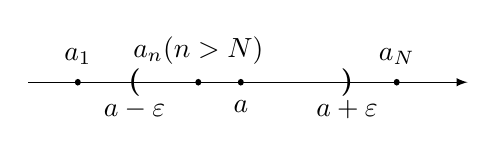
\begin{tikzpicture}[>=latex, xscale=0.9]
  \draw[->] (-3,0) -- (3.2,0);
  \node[above] at (-2.3,0.1) {$a_1$};
  \fill (-2.3,0) circle (1.2pt);
  \node at (-1.5,0) {\textbf{(}};
  \node[below=3pt] at (-1.5,0) {$a-\varepsilon$};
  \node[above] at (-0.6,0.1) {$a_n(n>N)$};
  \fill (-0.6,0) circle (1.2pt);
  \fill (0,0) circle (1.2pt);
  \node[below=3pt] at (0,0) {$a$};
  \node at (1.5,0) {\textbf{)}};
  \node[below=3pt] at (1.5,0) {$a+\varepsilon$};
  \node[above] at (2.2,0.1) {$a_N$};
  \fill (2.2,0) circle (1.2pt);
\end{tikzpicture}
\caption{}\label{fig:1.1.1}
\end{minipage}
\hfill
\begin{minipage}[t]{0.48\textwidth}
\centering
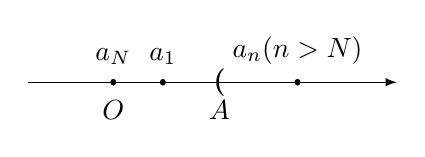
\begin{tikzpicture}[>=latex, xscale=0.9]
  \draw[->] (-1.2,0) -- (4,0);
  \fill (0,0) circle (1.2pt);
  \node[below=3pt] at (0,0) {$O$};
  \node[above] at (0,0.1) {$a_N$};
  \fill (0.7,0) circle (1.2pt);
  \node[above] at (0.7,0.1) {$a_1$};
  \node at (1.5,0) {\textbf{(}};
  \node[below=3pt] at (1.5,0) {$A$};
  \fill (2.6,0) circle (1.2pt);
  \node[above] at (2.6,0.1) {$a_n(n>N)$};
\end{tikzpicture}
\caption{}\label{fig:1.1.2}
\end{minipage}
\end{figure}

如果 $\forall A>0,\ \exists N=N(A)\in\mathbb{N}$, 当 $n>N$ 时, 有 $a_{n}<-A$, 则称 $-\infty$ 为数列 $\{a_{n}\}$ 的极限, 或称 $\{a_{n}\}$ 以 $-\infty$ 为极限, 或 $\{a_{n}\}$ 发散于 $-\infty$, 记为 $\lim_{n\to+\infty}a_{n}=-\infty$ 或 $a_{n}\to-\infty\ (n\to+\infty)$. 此时, 在 $(-\infty,-A)$ 外至多有 $a_{1},\cdots,a_{N}$ 中的 $N$ 项 (如图~\ref{fig:1.1.3} 所示).

如果 $\forall A>0,\ \exists N=N(A)\in\mathbb{N}$, 当 $n>N$ 时, 有
\[
  |a_{n}|>A,
\]
则称 $\infty$ 为数列 $\{a_{n}\}$ 的极限, 或称 $\{a_{n}\}$ 以 $\infty$ 为极限, 或 $\{a_{n}\}$ 发散于 $\infty$, 记为 $\lim_{n\to+\infty}a_{n}=\infty$ 或 $a_{n}\to\infty\ (n\to+\infty)$. 此时, 在 $(-\infty,-A)\cup(A,+\infty)$ 外, 即 $[-A,A]$ 中至多有 $a_{1},\cdots,a_{N}$ 中的 $N$ 项 (如图~\ref{fig:1.1.4} 所示).

\begin{figure}[htbp]
\centering
\begin{minipage}[t]{0.48\textwidth}
\centering
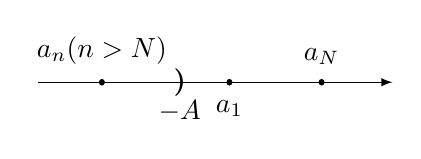
\begin{tikzpicture}[>=latex, xscale=0.9]
  \draw[->] (-3.5,0) -- (1.5,0);
  \fill (-2.6,0) circle (1.2pt);
  \node[above] at (-2.6,0.1) {$a_n(n>N)$};
  \node at (-1.5,0) {\textbf{)}};
  \node[below=3pt] at (-1.5,0) {$-A$};
  \fill (-0.8,0) circle (1.2pt);
  \node[below=3pt] at (-0.8,0) {$a_1$};
  \fill (0.5,0) circle (1.2pt);
  \node[above] at (0.5,0.1) {$a_N$};
\end{tikzpicture}
\caption{}\label{fig:1.1.3}
\end{minipage}
\hfill
\begin{minipage}[t]{0.48\textwidth}
\centering
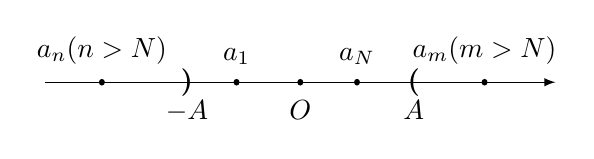
\begin{tikzpicture}[>=latex, xscale=0.9]
  \draw[->] (-3.6,0) -- (3.6,0);
  \fill (-2.8,0) circle (1.2pt);
  \node[above] at (-2.8,0.1) {$a_n(n>N)$};
  \node at (-1.6,0) {\textbf{)}};
  \node[below=3pt] at (-1.6,0) {$-A$};
  \fill (-0.9,0) circle (1.2pt);
  \node[above] at (-0.9,0.1) {$a_1$};
  \fill (0,0) circle (1.2pt);
  \node[below=3pt] at (0,0) {$O$};
  \fill (0.8,0) circle (1.2pt);
  \node[above] at (0.8,0.1) {$a_N$};
  \node at (1.6,0) {\textbf{(}};
  \node[below=3pt] at (1.6,0) {$A$};
  \fill (2.6,0) circle (1.2pt);
  \node[above] at (2.6,0.1) {$a_m(m>N)$};
\end{tikzpicture}
\caption{}\label{fig:1.1.4}
\end{minipage}
\end{figure}

综合上述各种情况可知, 一个数列 $\{a_n\}$ 或者收敛 (即 $\lim_{n\to+\infty}a_n=a\in\mathbb{R}$), 或者发散 (即 $\lim_{n\to+\infty}a_n=+\infty, -\infty, \infty$ 或无极限).

显然, 改变数列 $\{a_{n}\}$ 的有限多项, 或去掉有限多项, 或添加有限多项, 不会改变数列 $\{a_{n}\}$ 的收敛和发散性.

\begin{example}\label{ex:1.1.1}
对常数列 $\{a_{n}\}$, $a_{n} = a$, 有 $\lim_{n \to +\infty} a_{n} = \lim_{n \to +\infty} a = a$.
\end{example}
\begin{proof}
$\forall\varepsilon>0$, 取任意的自然数 $N$, 当 $n>N$ 时, 有
\[
  |a_{n}-a|=|a-a|=0<\varepsilon,
\]
所以 $\lim_{n\to+\infty}a_n=\lim_{n\to+\infty}a=a$.
\end{proof}

\begin{example}\label{ex:1.1.2}
$\lim_{n\to+\infty}\frac{1}{n^\alpha}=0\ (\alpha>0)$.
\end{example}
\begin{proof}
$\forall\varepsilon>0$, 取 $N\in\mathbb{N}$, s.\,t. (such that, 使得) $N>\left(\frac{1}{\varepsilon}\right)^{\frac{1}{\alpha}}$ 或者 $N=\left[\left(\frac{1}{\varepsilon}\right)^{\frac{1}{\alpha}}\right]+1$ (其中 $[x]$ 表示不超过 $x$ 的最大整数), 当 $n>N$ 时, 有
\[
  \left|\frac{1}{n^{\alpha}}-0\right|=\frac{1}{n^{\alpha}}<\frac{1}{N^{\alpha}}<\varepsilon,
\]
所以 $\lim_{n\to+\infty}\frac{1}{n^{\alpha}}=0$.

当 $\alpha=1$ 时, $\lim_{n\to+\infty}\frac{1}{n}=0$, 取 $N=\left[\frac{1}{\varepsilon}\right]+1$ (或 $N>\frac{1}{\varepsilon}, N\in\mathbb{N}$).
\end{proof}

\begin{example}\label{ex:1.1.3}
$\lim_{n\to+\infty}q^n=0\ (|q|<1)$.
\end{example}
\begin{proof}
\textit{证法 1}\quad 当 $0<|q|<1$ 时, $\frac{1}{|q|}>1$, 可设 $\frac{1}{|q|}=1+h\ (h>0)$. $\forall\varepsilon>0$, 取 $N\in\mathbb{N}$, s.\,t. $N>\frac{1}{\varepsilon h}$, 当 $n>N$ 时, 由二项式展开式知
\[
  \frac{1}{|q|^n}=(1+h)^n = 1+nh+\cdots+h^n > nh > Nh > \frac{1}{\varepsilon},
\]
即 $|q^n| < \varepsilon$. 于是
\[
  |q^n-0|=|q^n|<\varepsilon,
\]
所以 $\lim_{n\to+\infty}q^{n}=0$.

当 $q=0$ 时, 由例~\ref{ex:1.1.1} 知, $\lim_{n\to+\infty}q^{n}=\lim_{n\to+\infty}0=0$.

\textit{证法 2}\quad 当 $0<|q|<1$ 时, $\forall\varepsilon>0$, 取 $N\in\mathbb{N}$, s.\,t. $N>\log_{|q|}\varepsilon$, 当 $n>N$ 时, 有
\[
  |q^{n}-0|=|q^{n}|<|q|^{N}<\varepsilon,
\]
所以 $\lim_{n\to+\infty}q^n=0$.
\end{proof}

\begin{example}\label{ex:1.1.4}
证明:
\begin{enumerate}
  \item 当 $q>1$ 时, $\lim_{n\to+\infty}q^n=+\infty$;
  \item 当 $q<-1$ 时, $\lim_{n\to+\infty}q^n=\infty$;
  \item 当 $q=-1$ 时, 数列 $\{q^n\}$ 无极限.
\end{enumerate}
\end{example}
\begin{proof}
(1) 设 $q=1+h\ (h>0)$. $\forall A>0$, 取 $N\in\mathbb{N}$, s.\,t. $N>\frac{A}{h}$. 当 $n>N$ 时, 由二项式定理有
\[
  q^n=(1+h)^n = 1+nh+\cdots+h^n > nh > Nh > A,
\]
所以 $\lim_{n\to+\infty}q^n=+\infty$.

(2) 当 $q<-1$ 时, $|q|>1$. 仿 (1) 可证 $\lim_{n\to+\infty}|q|^n=+\infty$, 即 $\forall A>0,\ \exists N\in\mathbb{N}$, 当 $n>N$ 时, 有 $|q^n|=|q|^n>A$. 因此 $\lim_{n\to+\infty}q^n=\infty$.

(3) 此外, 当 $|q|<1$ 时, 由例~\ref{ex:1.1.3} 知 $\lim_{n\to+\infty}q^n=0$; 当 $q=1$ 时, 由例~\ref{ex:1.1.1} 知 $\lim_{n\to+\infty}q^n=\lim_{n\to+\infty}1=1$; 最后, 当 $q=-1$ 时, 由后面的例~\ref{ex:1.1.12} 推得 $\lim_{n\to+\infty}q^n$ 不存在.
\end{proof}

\begin{example}\label{ex:1.1.5}
设 $a$ 为实常数, 则 $\lim_{n\to+\infty}\frac{a^n}{n!}=0$.
\end{example}
\begin{proof}
显然, $\exists N_{0} \in \mathbb{N}$, s.\,t. $N_{0}>2|a|$, 即 $\frac{|a|}{N_0}<\frac{1}{2}$. 当 $n>N_0$ 时,
\begin{align*}
  \left|\frac{a^{n}}{n!}-0\right| &= \frac{|a|^{n}}{n!} = \frac{|a|}{1}\cdot\frac{|a|}{2}\cdots\frac{|a|}{N_{0}}\cdot\frac{|a|}{N_{0}+1}\cdots\frac{|a|}{n}\\
  &< \frac{|a|^{N_{0}}}{N_{0}!}\left(\frac{|a|}{N_{0}}\right)^{n-N_{0}} < \frac{|a|^{N_{0}}}{N_{0}!}\left(\frac{1}{2}\right)^{n-N_{0}} = C\left(\frac{1}{2}\right)^{n},
\end{align*}
其中 $C = \frac{|a|^{N_0}}{N_0!}\cdot 2^{N_0}$ 为与 $n$ 无关的常数.

由例~\ref{ex:1.1.3} 知, $\lim_{n\to+\infty}\left(\frac{1}{2}\right)^{n}=0$. 故 $\forall\varepsilon>0,\ \exists N_{1}\in\mathbb{N}$, 当 $n>N_1$ 时, 有 $\left(\frac{1}{2}\right)^{n}<\frac{\varepsilon}{C}$. 取 $N=\max\{N_0, N_1\}$, 当 $n>N$ 时, 有
\[
  \left|\frac{a^n}{n!}-0\right| < C\left(\frac{1}{2}\right)^n < C\cdot\frac{\varepsilon}{C}=\varepsilon,
\]
所以 $\lim_{n\to+\infty}\frac{a^n}{n!}=0$.
\end{proof}

\begin{example}\label{ex:1.1.6}
$\lim_{n\to+\infty}\sqrt[n]{a}=\lim_{n\to+\infty}a^{\frac{1}{n}}=1\ (a>0)$.
\end{example}
\begin{proof}
\textit{证法 1}\quad 当 $a=1$ 时, 由例~\ref{ex:1.1.1} 可知 $\lim_{n\to+\infty}\sqrt[n]{a}=\lim_{n\to+\infty}1=1$.

当 $a>1$ 时, $\sqrt[n]{a}>1$. 令 $\sqrt[n]{a}=1+\alpha_n\ (\alpha_n>0)$, 则
\[
  a = (1+\alpha_n)^n = 1+n\alpha_n+\cdots+\alpha_n^n > n\alpha_n,
\]
即 $0<\alpha_n<\frac{a}{n}$. $\forall\varepsilon>0$, 取 $N>\left[\frac{a}{\varepsilon}\right]$, 当 $n>N$ 时, 有
\[
  |\sqrt[n]{a}-1| = \alpha_n < \frac{a}{n} < \frac{a}{N} < \varepsilon,
\]
所以 $\lim_{n\to+\infty}\sqrt[n]{a}=1$.

当 $0<a<1$ 时, $\frac{1}{a}>1$. 由上面已证的结果, $\lim_{n\to+\infty}\sqrt[n]{\frac{1}{a}}=1$, 从而
\[
  \lim_{n\to+\infty}\sqrt[n]{a}=\lim_{n\to+\infty}\frac{1}{\sqrt[n]{\frac{1}{a}}}=1.
\]

\textit{证法 2}\quad 当 $a>1$ 时, $\forall\varepsilon>0$, 只要取 $N\in\mathbb{N}$, s.\,t. $N>\log_{1+\varepsilon}a$, 当 $n>N$ 时, 便有
\[
  1 \leqslant \sqrt[n]{a} < \sqrt[N]{a} < 1+\varepsilon,
\]
即 $|\sqrt[n]{a}-1|<\varepsilon$. 故 $\lim_{n\to+\infty}\sqrt[n]{a}=1$. $a\leqslant 1$ 的情形同证法 1.
\end{proof}

\begin{example}\label{ex:1.1.7}
$\lim_{n\to+\infty}\sqrt[n]{n}=1$.
\end{example}
\begin{proof}
\textit{证法 1}\quad 令 $\sqrt[n]{n}=1+\alpha_{n}\ (\alpha_{n}\geqslant0)$, 则当 $n>1$ 时,
\[
  n = (1+\alpha_{n})^{n} = 1+n\alpha_{n}+\frac{n(n-1)}{2}\alpha_{n}^{2}+\cdots+\alpha_{n}^{n} > \frac{n(n-1)}{2}\alpha_{n}^{2},
\]
从而 $\alpha_n^2 < \frac{2}{n-1}$, 即 $0 \leqslant \alpha_n < \sqrt{\frac{2}{n-1}}$.

$\forall\varepsilon>0$, 取 $N = \left[\frac{2}{\varepsilon^2}\right]+1$, 当 $n>N$ 时, 有
\[
  |\sqrt[n]{n}-1| = \alpha_n < \sqrt{\frac{2}{n-1}} < \sqrt{\frac{2}{N-1}} \leqslant \varepsilon,
\]
所以 $\lim_{n\to+\infty}\sqrt[n]{n}=1$.

\textit{证法 2}\quad $\forall\varepsilon>0$, 取充分大的自然数 $k$, 使 $(1+\varepsilon)^k > 2$. 当 $n>2^k$ 时,
\[
  1 \leqslant \sqrt[n]{n} < \sqrt[n]{(1+\varepsilon)^n} = 1+\varepsilon,
\]
所以 $\lim_{n\to+\infty}\sqrt[n]{n}=1$.
\end{proof}

\begin{example}\label{ex:1.1.8}
设 $a_{n}=0.\underbrace{33\cdots3}_n$, 则 $\lim_{n\to+\infty}a_{n}=\frac{1}{3}$.
\end{example}
\begin{proof}
因为
\[
  a_{n} = \frac{3}{10}+\frac{3}{10^2}+\cdots+\frac{3}{10^n} = \frac{\frac{3}{10}\left(1-\frac{1}{10^n}\right)}{1-\frac{1}{10}} = \frac{1}{3}\left(1-\frac{1}{10^n}\right),
\]
所以
\[
  \left|a_{n}-\frac{1}{3}\right| = \frac{1}{3\cdot 10^n} < \frac{1}{10^n}.
\]
$\forall\varepsilon>0$, 取 $N = \left[\lg\frac{1}{\varepsilon}\right]+1$, 当 $n>N$ 时, 有
\[
  \left|a_{n}-\frac{1}{3}\right| < \frac{1}{10^n} < \frac{1}{10^N} \leqslant \varepsilon,
\]
所以 $\lim_{n\to+\infty}a_{n}=\frac{1}{3}$.
\end{proof}

\begin{example}\label{ex:1.1.9}
$\lim_{n \to +\infty} \frac{1}{n \sqrt[n]{n!}} = 0$.
\end{example}
\begin{proof}
\textit{证法 1}\quad $\forall\varepsilon>0$, 由例~\ref{ex:1.1.5} 知 $\lim_{n\to+\infty}\frac{(1/\varepsilon)^n}{n!}=0$. 故 $\exists N\in\mathbb{N}$, 当 $n>N$ 时, 有
\[
  \frac{(1/\varepsilon)^{n}}{n!}<1,
\]
所以
\[
  -\varepsilon < 0 < \frac{1}{\sqrt[n]{n!}} < \varepsilon,
\]
即 $\lim_{n\to+\infty}\frac{1}{\sqrt[n]{n!}}=0$. 进而由 $n\geqslant 1$ 知
\[
  0 < \frac{1}{n\sqrt[n]{n!}} \leqslant \frac{1}{\sqrt[n]{n!}} < \varepsilon,
\]
所以 $\lim_{n\to+\infty}\frac{1}{n\sqrt[n]{n!}}=0$.

\textit{证法 2}\quad 容易验证不等式 $n! > \left(\frac{n}{e}\right)^n$ (可参阅例~\ref{ex:1.4.11}). 从而
\[
  0 < \frac{1}{n\sqrt[n]{n!}} < \frac{e}{n^2}.
\]
$\forall\varepsilon>0$, 取 $N = \left[\sqrt{\frac{e}{\varepsilon}}\right]+1$, 当 $n>N$ 时即有 $\frac{e}{n^2}<\varepsilon$, 故极限为 0.
\end{proof}

\begin{example}\label{ex:1.1.10}
$\lim_{n\to+\infty}\frac{3n^{2}}{n^{2}-3}=3$.
\end{example}
\begin{proof}
当 $n\geqslant 2$ 时, $n^2-3 > \frac{n^2}{2}$. 故
\[
  \left|\frac{3n^{2}}{n^{2}-3}-3\right| = \frac{9}{n^{2}-3} < \frac{18}{n^{2}}.
\]
$\forall\varepsilon>0$, 取 $N = \max\left\{2, \left[\sqrt{\frac{18}{\varepsilon}}\right]+1\right\}$, 当 $n>N$ 时, 有
\[
  \left|\frac{3n^{2}}{n^{2}-3}-3\right| < \frac{18}{n^2} < \frac{18}{N^2} \leqslant \varepsilon,
\]
所以 $\lim_{n\to+\infty}\frac{3n^{2}}{n^{2}-3}=3$.
\end{proof}

\begin{example}\label{ex:1.1.11}
$\lim_{n \to +\infty} \frac{3 \sqrt{n} + 1}{2 \sqrt{n} + n} = 0$.
\end{example}
\begin{proof}
$\forall\varepsilon>0$, 当 $n\geqslant 1$ 时,
\[
  \left|\frac{3\sqrt{n}+1}{2\sqrt{n}+n}-0\right| = \frac{3\sqrt{n}+1}{2\sqrt{n}+n} < \frac{4\sqrt{n}}{n} = \frac{4}{\sqrt{n}}.
\]
取 $N = \left[\frac{16}{\varepsilon^2}\right]+1$, 当 $n>N$ 时, 有
\[
  \left|\frac{3\sqrt{n}+1}{2\sqrt{n}+n}-0\right| < \frac{4}{\sqrt{n}} < \frac{4}{\sqrt{N}} \leqslant \varepsilon,
\]
所以 $\lim_{n\to+\infty}\frac{3\sqrt{n}+1}{2\sqrt{n}+n}=0$.
\end{proof}

\begin{theorem}\label{thm:1.1.1}
数列 $\{a_{n}\}$ 有极限 $a$ 的充分必要条件是它的偶数项数列 (偶子列) $\{a_{2k}\}$ 和奇数项数列 (奇子列) $\{a_{2k-1}\}$ 都有极限且极限均为 $a$.
\end{theorem}
\begin{proof}
\textbf{必要性:}\quad 设 $\lim_{n\to+\infty}a_n=a$.

若 $a$ 为有限实数, 则 $\forall\varepsilon>0,\ \exists N\in\mathbb{N}$, 当 $n>N$ 时, 有 $|a_n-a|<\varepsilon$. 特别地, 取自然数 $K = \left[\frac{N}{2}\right]+1$, 当 $k>K$ 时, $2k>2k-1>N$, 因而
\[
  |a_{2k}-a|<\varepsilon\quad \text{与}\quad |a_{2k-1}-a|<\varepsilon,
\]
即 $\lim_{k\to+\infty}a_{2k}=a$ 且 $\lim_{k\to+\infty}a_{2k-1}=a$.

对 $a=+\infty, -\infty, \infty$ 的情形完全类似可证.

\textbf{充分性:}\quad 设 $\lim_{k\to+\infty}a_{2k}=a$ 且 $\lim_{k\to+\infty}a_{2k-1}=a$.

若 $a$ 为有限实数, 则 $\forall\varepsilon>0$, $\exists K_1\in\mathbb{N}$, 当 $k>K_1$ 时, $|a_{2k}-a|<\varepsilon$; $\exists K_2\in\mathbb{N}$, 当 $k>K_2$ 时, $|a_{2k-1}-a|<\varepsilon$. 取 $N = \max\{2K_1, 2K_2-1\}$, 则当 $n>N$ 时, 无论 $n$ 是偶数 ($n=2k>2K_1$) 还是奇数 ($n=2k-1>2K_2-1$), 都有 $|a_n-a|<\varepsilon$. 故 $\lim_{n\to+\infty}a_n=a$.

对 $a=+\infty, -\infty, \infty$ 的情形同理可证.
\end{proof}

下面引进开邻域的概念:
\begin{enumerate}
  \item 设 $a\in\mathbb{R}$, 称开区间 $(a-\varepsilon, a+\varepsilon)$ 为点 $a$ 的 $\varepsilon$ 邻域, 记作 $U(a;\varepsilon)$ 或简记为 $U(a)$. 称集合 $U^\circ(a;\varepsilon) = (a-\varepsilon, a)\cup(a, a+\varepsilon)$ 为点 $a$ 的去心邻域.
  \item 称开区间 $(A, +\infty)$ 为点 $+\infty$ 的开邻域, 记作 $U(+\infty; A)$ 或 $U(+\infty)$.
  \item 称开区间 $(-\infty, -A)$ 为点 $-\infty$ 的开邻域, 记作 $U(-\infty; A)$ 或 $U(-\infty)$.
  \item 称开集 $(-\infty, -A)\cup(A, +\infty)$ 为点 $\infty$ 的开邻域, 记作 $U(\infty; A)$ 或 $U(\infty)$.
\end{enumerate}

由开邻域的概念, 数列极限的定义可以统一叙述为:
\[
  \lim_{n\to+\infty}a_n = a \iff \text{对 } a \text{ 的任何开邻域 } U,\ \exists N\in\mathbb{N},\ \text{当 } n>N \text{ 时, } a_n\in U.
\]

\begin{theorem}\label{thm:1.1.2}
$\lim_{n\to+\infty}a_n=a \iff$ 对 $\{a_n\}$ 的任何子列 $\{a_{n_k}\}$ 都有 $\lim_{k\to+\infty}a_{n_k}=a$.
\end{theorem}
\begin{proof}
\textbf{充分性:}\quad 因为数列 $\{a_n\}$ 本身就是它的一个平凡子列 (取 $n_k=k$), 所以结论显然成立.

\textbf{必要性:}\quad 设 $\lim_{n\to+\infty}a_n=a$. 对 $a$ 的任何开邻域 $U$, $\exists N\in\mathbb{N}$, 当 $n>N$ 时, $a_n\in U$. 因为子列的下标序列 $\{n_k\}$ 严格递增, 且 $n_k\geqslant k$, 所以当 $k>N$ 时必有 $n_k\geqslant k>N$, 从而 $a_{n_k}\in U$. 故 $\lim_{k\to+\infty}a_{n_k}=a$.
\end{proof}

\begin{theorem}\label{thm:1.1.3}
数列 $\{a_{n}\}$ 有极限 (实数 $a$ 或 $+\infty$ 或 $-\infty$) 的充要条件是它的任何非平凡子列都有极限.
\end{theorem}
\begin{proof}
必要性由定理~\ref{thm:1.1.2} 直接保证. 充分性反设 $\{a_n\}$ 没有极限, 则由极限否定定义可析出两个极限不同的子列, 矛盾.
\end{proof}

\begin{theorem}\label{thm:1.1.4}
数列 $\{a_{n}\}$ 收敛 $\iff \{a_{n}\}$ 的任何非平凡子列都收敛.
\end{theorem}

\begin{theorem}\label{thm:1.1.5}
$\lim_{n \to +\infty} a_n = a \iff a$ 的任何开邻域 $U$ 的外边 $\mathbb{R} \setminus U$ 中至多含有限项.
\end{theorem}
\begin{proof}
\textbf{必要性:}\quad 由极限定义, 当 $n>N$ 时 $a_n\in U$, 故在 $U$ 外部至多只有 $a_1, a_2, \cdots, a_N$ 这有限多项.

\textbf{充分性:}\quad 对任何开邻域 $U$, 若 $U$ 外面只有有限项, 设这些项的最大下标为 $N$ (若外面无项则取 $N=1$), 则当 $n>N$ 时必有 $a_n\in U$, 从而 $\lim_{n\to+\infty}a_n=a$.
\end{proof}

\begin{example}\label{ex:1.1.12}
数列 $\{a_{n}\}$, $a_{n} = (-1)^{n-1}$ 无极限, 当然不收敛.
\end{example}
\begin{proof}
\textit{证法 1}\quad 它的奇子列 $a_{2k-1} = 1 \to 1$, 偶子列 $a_{2k} = -1 \to -1$. 由定理~\ref{thm:1.1.1} 或定理~\ref{thm:1.1.2} 知, $(-1)^{n-1}$ 无极限.

\textit{证法 2}\quad $\forall a\neq\pm 1$, 取 $\varepsilon_{0}=\min\{|a-1|, |a+1|\}>0$, 则数列 $(-1)^{n-1}$ 全部各项都在开邻域 $U=(a-\varepsilon_0, a+\varepsilon_0)$ 的外部.
当 $a=1$ 时, $-1=(-1)^{2k}$ 全在 $1$ 的开邻域 $U=(1-1/2, 1+1/2)=(1/2, 3/2)$ 外部;
当 $a=-1$ 时, $1=(-1)^{2k-1}$ 全在 $-1$ 的开邻域 $U=(-3/2, -1/2)$ 外部;
当 $a=+\infty$ 时, 全在 $U=(1, +\infty)$ 外部;
当 $a=-\infty$ 时, 全在 $U=(-\infty, -1)$ 外部;
当 $a=\infty$ 时, 全在 $U=(-\infty, -1)\cup(1, +\infty)$ 外部.
根据定理~\ref{thm:1.1.5}, 任何数及 $\pm\infty, \infty$ 均不为该数列极限.
\end{proof}

\begin{example}\label{ex:1.1.13}
数列 $\{\sin n\}$ 无极限.
\end{example}
\begin{proof}
$\forall k\in\mathbb{N}$, 区间 $\left(2k\pi+\frac{\pi}{4}, 2k\pi+\frac{3\pi}{4}\right)$ 的长度为 $\frac{\pi}{2}>1$, 故必存在自然数 $n_{k}\in\left(2k\pi+\frac{\pi}{4}, 2k\pi+\frac{3\pi}{4}\right)\cap\mathbb{N}$. 同理, 区间 $((2k-1)\pi, 2k\pi)$ 的长度为 $\pi>1$, 必存在自然数 $n_{k}'\in((2k-1)\pi, 2k\pi)\cap\mathbb{N}$ (如图~\ref{fig:1.1.5} 所示).

\begin{figure}[htbp]
\centering
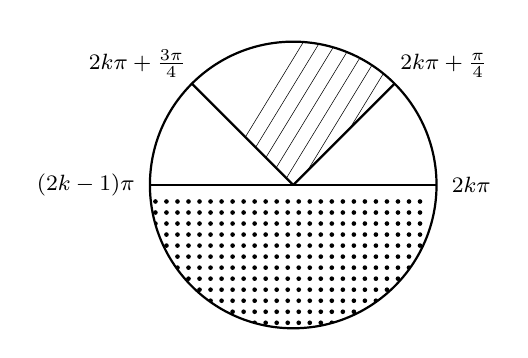
\begin{tikzpicture}[>=latex, scale=1.4]
  % 扇形斜线阴影
  \begin{scope}
    \clip (0,0) -- (45:1.3) arc (45:135:1.3) -- cycle;
    \foreach \x in {-1.8,-1.65,...,1.8} {
      \draw[very thin] (\x,-1.8) -- (\x+2.2,1.8);
    }
  \end{scope}
  % 下半圆点阵阴影
  \begin{scope}
    \clip (-1.3,0) arc (180:360:1.3) -- cycle;
    \foreach \x in {-1.25,-1.15,...,1.25} {
      \foreach \y in {-1.25,-1.15,...,-0.05} {
        \fill (\x,\y) circle (0.6pt);
      }
    }
  \end{scope}
  % 轮廓与分割线
  \draw[thick] (0,0) circle (1.3);
  \draw[thick] (-1.3,0) -- (1.3,0);
  \draw[thick] (0,0) -- (45:1.3);
  \draw[thick] (0,0) -- (135:1.3);
  % 标注
  \node[left=2pt] at (-1.3,0) {\footnotesize $(2k-1)\pi$};
  \node[right=2pt] at (1.3,0) {\footnotesize $2k\pi$};
  \node[above left] at (135:1.25) {\footnotesize $2k\pi+\frac{3\pi}{4}$};
  \node[above right] at (45:1.25) {\footnotesize $2k\pi+\frac{\pi}{4}$};
\end{tikzpicture}
\caption{}\label{fig:1.1.5}
\end{figure}

显然 $n_1<n_2<\cdots$ 且 $n_1'<n_2'<\cdots$. 对于子列 $\{a_{n_k}\}$, 有
\[
  a_{n_k} = \sin n_k > \sin\frac{\pi}{4} = \frac{\sqrt{2}}{2};
\]
而对于子列 $\{a_{n_k'}\}$, 有
\[
  a_{n_k'} = \sin n_k' < 0.
\]
故若极限存在为 $a$, 则必然有 $a\geqslant\frac{\sqrt{2}}{2}$ 且 $a\leqslant 0$, 矛盾! 故数列 $\{\sin n\}$ 无极限.
\end{proof}

\begin{theorem}[保号性与保序性]\label{thm:1.1.6}
设 $\lim_{n\to+\infty} a_n = a > b$ (或 $<b$), 则 $\exists N_0 \in \mathbb{N}$, 当 $n>N_0$ 时有 $a_n > b$ (或 $a_n < b$).
\end{theorem}
\begin{proof}
取 $\varepsilon = a-b > 0$. 由极限定义, $\exists N_0\in\mathbb{N}$, 当 $n>N_0$ 时, 有
\[
  |a_n-a| < \varepsilon \implies a_n > a-\varepsilon = a-(a-b) = b.
\]
同理可证 $a<b$ 的情形.
\end{proof}

\begin{example}\label{ex:1.1.14}
设 $\lim_{n\to+\infty}a_n=0$ (极限为 0 的变量称为无穷小量), 且数列 $\{b_n\}$ 有界 (即 $\exists M>0$ 使 $|b_n|\leqslant M$), 则
\[
  \lim_{n\to+\infty}a_n b_n = 0.
\]
即无穷小量与有界变量之积仍为无穷小量.
\end{example}
\begin{proof}
$\forall\varepsilon>0$, 因 $\lim_{n\to+\infty}a_n=0$, 故 $\exists N\in\mathbb{N}$, 当 $n>N$ 时, 有 $|a_n-0|<\frac{\varepsilon}{M+1}$. 于是
\[
  |a_{n}b_{n}-0|=|a_{n}b_{n}|\leqslant M|a_{n}| \leqslant M\cdot\frac{\varepsilon}{M+1}<\varepsilon,
\]
所以 $\lim_{n\to+\infty}a_n b_n = 0$.
\end{proof}

\begin{example}[Ces\`aro 算术平均]\label{ex:1.1.15}
设 $\lim_{n\to+\infty}a_n=a$ (实数, $+\infty, -\infty$), 则
\[
  \lim_{n\to+\infty}\frac{a_1+a_2+\cdots+a_n}{n}=a.
\]
但反之不真.
\end{example}
\begin{proof}
反之不真显见: 取 $a_n=(-1)^{n-1}$, 则 $\{a_n\}$ 发散, 但 $\frac{a_1+\cdots+a_n}{n}\to 0$.

现在证明正向结论:
当 $a\in\mathbb{R}$ 时, 设 $a_n = a+\alpha_n$, 其中 $\lim_{n\to+\infty}\alpha_n=0$. 则
\[
  \frac{a_1+\cdots+a_n}{n} = a + \frac{\alpha_1+\cdots+\alpha_n}{n}.
\]
$\forall\varepsilon>0$, $\exists N_1\in\mathbb{N}$, 当 $n>N_1$ 时, $|\alpha_n|<\frac{\varepsilon}{2}$. 取定 $N_1$ 后, $\sum_{k=1}^{N_1}|\alpha_k|$ 为常数, 故 $\exists N_2>N_1$, 当 $n>N_2$ 时, $\frac{\sum_{k=1}^{N_1}|\alpha_k|}{n}<\frac{\varepsilon}{2}$. 于是当 $n>N_2$ 时,
\[
  \left|\frac{\alpha_1+\cdots+\alpha_n}{n}\right| \leqslant \frac{\sum_{k=1}^{N_1}|\alpha_k|}{n} + \frac{\sum_{k=N_1+1}^n|\alpha_k|}{n} < \frac{\varepsilon}{2} + \frac{(n-N_1)\frac{\varepsilon}{2}}{n} < \varepsilon.
\]
故 $\lim_{n\to+\infty}\frac{a_1+\cdots+a_n}{n}=a$.

当 $a=+\infty$ 时, $\forall A>0$, $\exists N_1\in\mathbb{N}$, 当 $n>N_1$ 时, $a_n > 2A+2$. 固定 $N_1$, 因 $\lim_{n\to+\infty}\frac{n-N_1}{n}=1>\frac{1}{2}$ 且 $\lim_{n\to+\infty}\frac{a_1+\cdots+a_{N_1}}{n}=0>-1$, 故 $\exists N_2>N_1$, 当 $n>N_2$ 时, 有
\[
  \frac{a_1+\cdots+a_n}{n} = \frac{a_1+\cdots+a_{N_1}}{n} + \frac{a_{N_1+1}+\cdots+a_n}{n} > -1 + \frac{n-N_1}{n}(2A+2) > -1 + \frac{1}{2}(2A+2) = A.
\]
故 $\lim_{n\to+\infty}\frac{a_1+\cdots+a_n}{n}=+\infty$.

$a=-\infty$ 的情形完全类似可证.
\end{proof}

\begin{example}\label{ex:1.1.16}
数列 $\{a_{n}\}$ 无上界 $\iff \{a_{n}\}$ 必有子列 $\{a_{n_{k}}\}$ 使得 $\lim_{k\to+\infty}a_{n_k}=+\infty$.
\end{example}
\begin{proof}
\textbf{充分性:}\quad 若有子列 $a_{n_k}\to+\infty$, 则对任意 $M>0$, 存在 $K$ 使得当 $k>K$ 时 $a_{n_k}>M$, 故原数列无上界.

\textbf{必要性:}\quad 设 $\{a_n\}$ 无上界. 取 $k=1$, $\exists n_1\in\mathbb{N}$ 使 $a_{n_1}>1$.
假设已选出 $n_1<n_2<\cdots<n_{k-1}$ 满足 $a_{n_j}>j\ (j=1,\cdots,k-1)$. 令
\[
  M_k = \max\{k, a_1, a_2, \cdots, a_{n_{k-1}}\}.
\]
因为 $\{a_n\}$ 无上界, 故必存在 $n_k$ 使得 $a_{n_k}>M_k$. 显然 $a_{n_k}>k$, 且由 $a_{n_k}>M_k \geqslant a_i\ (1\leqslant i\leqslant n_{k-1})$ 可知 $n_k > n_{k-1}$.
以此归纳可得子列 $\{a_{n_k}\}$, 满足 $n_1<n_2<\cdots$ 且 $a_{n_k}>k$. 故 $\lim_{k\to+\infty}a_{n_k}=+\infty$.
\end{proof}

\begin{exblock}{练习题 1.1}
\item 用数列极限定义证明:
\begin{enumerate}
  \item $\lim_{n \to +\infty} 0.\underbrace{99 \cdots 9}_n = 1$;
  \item $\lim_{n \to +\infty} \frac{3n + 4}{7n - 3} = \frac{3}{7}$;
  \item $\lim_{n \to +\infty} \frac{5n + 6}{n^2 - n - 1000} = 0$;
  \item $\lim_{n \to +\infty} \frac{8}{2^n + 5} = 0$;
  \item $\lim_{n \to +\infty} \frac{\sin n!}{n^{1/2}} = 0$;
  \item $\lim_{n \to +\infty} (\sqrt{n + 2} - \sqrt{n - 2}) = 0$;
  \item $\lim_{n \to +\infty} (\sqrt[3]{n+2} - \sqrt[3]{n-2}) = 0$;
  \item $\lim_{n \to +\infty} \frac{n^{3/2} \arctan n}{1 + n^2} = 0$;
  \item $\lim_{n \to +\infty} a_n = 1$, 其中 $a_n = \begin{cases} \frac{n-1}{n}, & n \text{ 为偶数}, \\ \frac{\sqrt{n^2 + n}}{n}, & n \text{ 为奇数}; \end{cases}$
  \item $\lim_{n \to +\infty} (n^3 - 4n - 5) = +\infty$.
\end{enumerate}

\item 设 $\lim_{n\to+\infty}a_n=a$. 证明: $\forall k\in\mathbb{N}$, 有 $\lim_{n\to+\infty}a_{n+k}=a$.

\item 设 $\lim_{n\to+\infty}a_n=a$. 证明: $\lim_{n\to+\infty}|a_n|=|a|$. 举例说明, 这个命题的逆命题不真.

\item 设 $x_{n} \leqslant a \leqslant y_{n}, n \in \mathbb{N}$, 且 $\lim_{n\to+\infty}(y_{n}-x_{n})=0$. 证明:
\[
  \lim_{n\to+\infty}x_{n}=\lim_{n\to+\infty}y_{n}=a.
\]

\item 设 $\{a_{n}\}$ 为一个收敛数列. 证明: 数列 $\{a_{n}\}$ 中或者有最大的数, 或者有最小的数. 举出两者都有的例子; 再举出只有一个的例子.

\item 证明下列数列发散:
\begin{enumerate}
  \item $\{n^{(-1)^n}\}$;
  \item $\{\cos n\}$.
\end{enumerate}

\item 证明: 数列 $\{a_{n}\}$ 收敛 $\iff$ 三个数列 $\{a_{3k-2}\}$, $\{a_{3k-1}\}$, $\{a_{3k}\}$ 都收敛且有相同的极限.

\item 设 $\lim_{n\to+\infty}(a_{n}-a_{n-1})=d$. 证明: $\lim_{n\to+\infty}\frac{a_n}{n}=d$.

\item 设 $\lim_{n\to+\infty} a_n = a$. 用 $\varepsilon\text{-}N$ 法, $A\text{-}N$ 法证明:
\[
  \lim_{n\to+\infty}\frac{a_1+2a_2+\cdots+na_n}{n^2}=\frac{a}{2}\quad (a \text{ 为实数}, +\infty, -\infty).
\]
\end{exblock}

\begin{exblock}{思考题 1.1}
\item 设 $\lim_{n\to+\infty}a_n=a$, $|q| < 1$. 用 $\varepsilon\text{-}N$ 法证明:
\[
  \lim_{n\to+\infty}(a_{n}+a_{n-1}q+\cdots+a_{1}q^{n-1})=\frac{a}{1-q}.
\]

\item 设 $\lim_{n\to+\infty}a_n=a$, $\lim_{n\to+\infty}b_n=b$. 用 $\varepsilon\text{-}N$ 法证明:
\[
  \lim_{n\to+\infty}\frac{a_0b_n+a_1b_{n-1}+\cdots+a_{n-1}b_1+a_nb_0}{n}=ab.
\]

\item 设 $\lim_{n\to+\infty}a_n=a, b_n\geqslant 0\ (n\in\mathbb{N}), \lim_{n\to+\infty}(b_1+b_2+\cdots+b_n)=S$. 证明:
\[
  \lim_{n\to+\infty}(a_nb_1+a_{n-1}b_2+\cdots+a_1b_n)=aS.
\]

\item \textbf{(Toeplitz 定理)}\ 设 $n, k \in \mathbb{N}$, $t_{nk} \geqslant 0$ 且 $\sum_{k=1}^{n} t_{nk} = 1$, $\lim_{n \to +\infty} t_{nk} = 0$. 如果 $\lim_{n \to +\infty} a_n = a$, 证明:
\[
  \lim_{n \to +\infty} \sum_{k=1}^{n} t_{nk} a_k = a.
\]
说明例~\ref{ex:1.1.15} 为 Toeplitz 定理的特殊情形.

\item 设 $a, b, c$ 为三个给定的实数, 令 $a_{0} = a, b_{0} = b, c_{0} = c$, 并归纳定义
\[
  \begin{cases}
    a_{n}=\dfrac{b_{n-1}+c_{n-1}}{2},\\[6pt]
    b_{n}=\dfrac{c_{n-1}+a_{n-1}}{2}, & n = 1, 2, \cdots.\\[6pt]
    c_{n}=\dfrac{a_{n-1}+b_{n-1}}{2},
\end{cases}
\]
证明: $\lim_{n\to+\infty}a_n=\lim_{n\to+\infty}b_n=\lim_{n\to+\infty}c_n=\frac{a+b+c}{3}$.

\item 设 $a_{1}, a_{2}$ 为实数, 令
\[
  a_{n}=pa_{n-1}+qa_{n-2},\quad n=3, 4, 5, \cdots,
\]
其中 $p > 0, q > 0, p + q = 1$. 证明: 数列 $\{a_{n}\}$ 收敛, 且 $\lim_{n \to +\infty} a_{n} = \frac{a_{2} + a_{1} q}{1 + q}$.

\item 设数列 $\{a_{n}\}$, $\{b_{n}\}$, $\{c_{n}\}$ 满足 $a_{1} > 0, 4 \leqslant b_{n} \leqslant 5, 4 \leqslant c_{n} \leqslant 5$,
\[
  a_{n}=\frac{\sqrt{b_{n}^{2}+c_{n}^{2}}}{b_{n}+c_{n}}a_{n-1}.
\]
证明: $\lim_{n\to+\infty}a_n = 0$.
\end{exblock}
